\section{Android Architecture Security}
This section details the overall architecture of the Android OS and various security concerns at each level.
The operating system is composed of five major layers that facilitate access to the hardware components and software services provided by the OS.
Figure \ref{fig:AndroidArch} shows Android's architecture model by layer and is pulled directly from the Android developer documentation \cite{AndroidDocs2022Arch}.

\begin{figure}[htbp]
    \centerline{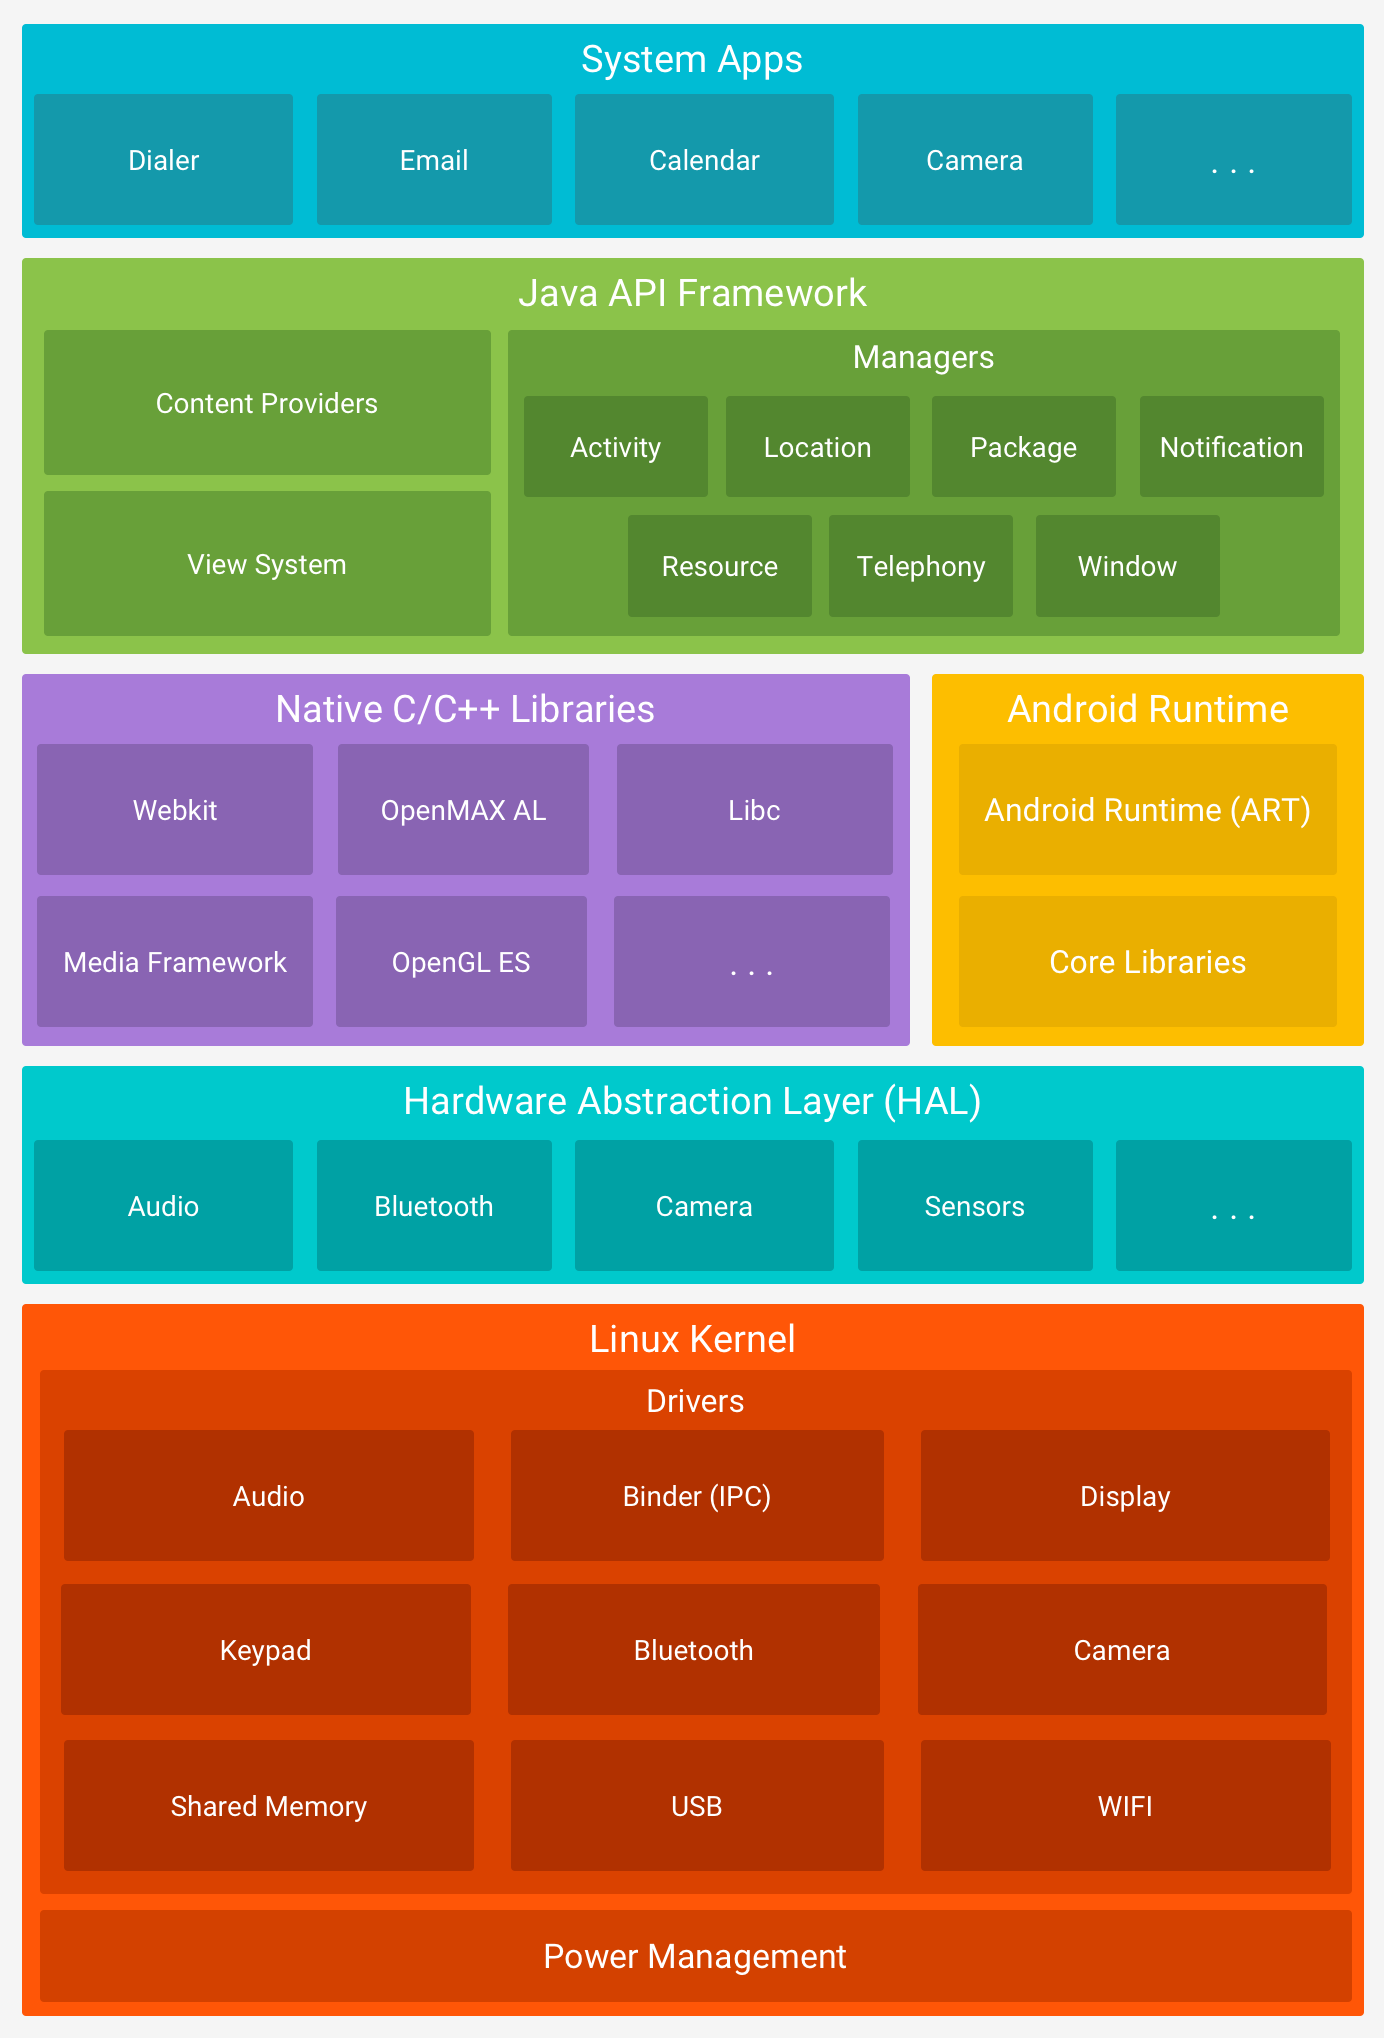
\includegraphics[width=0.4\textwidth]{figures/AndroidArch.png}}
    \caption{Android architecture model.}
    \label{fig:AndroidArch}
\end{figure}

Linares-Vasquez \etal breaks downs the vulnerabilities affecting the Android system \cite{LinaresVasquez2017}.
A majority of vulnerabilities occur at the lowest level of abstraction for the Android architecture model: the Linux kernel layer.
The next highest share of vulnerabilities exist within the native libraries supported by the Android platform.
These two portions of the Android architecture account for roughly 73\% of the sampled vulnerabilities studied.
This study provides a good overview of the distribution of vulnerabilities that exist in the Android platform.

\subsection{The Linux Kernel Layer}
The lowest part of the architecture stack is the Linux kernel that Android derived from.
The primary benefit of building an OS based on a Linux kernel is the maintenance performed on the Linux kernel by Linux developers.
In the case of Android, the overwhelming majority of bug fixes (95\%) are the result of work done by the Linux kernel development team \cite{Khomh2012}.

Another benefit of basing an OS on the Linux kernel is the wide range of functional OS support provided by the kernel already.
The adapted version of the Linux kernel used as the foundation to build the Android OS employs preexisting kernel features.
Most changes made to the Linux kernel adapted for Android extend current kernel functions or employ new features that make the OS more suitable for use on mobile devices, such as a more aggressive memory manager used to preserve the limited memory resources on the device and a power manager \cite{AndroidDocs2022Arch, Khomh2012}.

Linux kernel development, at the time of version 2.6, was carried out by a large group of developers from a multitude of different organizations and from developers acting independently \cite{KroahHartman2007}.
A significant portion of the kernel was dedicated to driver and architecture support, which is code that interfaces and provides hardware support.
This large pool of developers doesn't explicitly increase the safety of the software, since there is no substantial evidence to support the claim that open source software is more secure than a proprietary counterpart \cite{Schryen2009, Witten2001}.
Instead, the open source nature of the Linux kernel facilitates three key points:
\begin{itemize}
    \item Organizations may develop drivers for their own hardware and maintain a measure of control over their own hardware security as a result. More generally, users have direct control when improving security of open source systems.
    \item Organizations and their developers may trust open source software more than a proprietary alternative.
    \item Organizations and their developers gain access to new features of the kernel approved by the maintainers of the source code.
\end{itemize}

The last point is particularly pertinent.
The earliest versions of Android were based on the Linux kernel 2.6 versions \cite{Gilski2015}.
These versions of the Linux kernel introduced the Linux Security Modules (LSM), which is a framework for general purpose access control \cite{Wright2002}.
The LSM explicitly supports the implementation of different security models that already existed at the time the feature was introduced, without favoring one over the other.
A notable example would be SELinux, which is an extensive, non-discretionary access control implementation contracted by the National Security Agency (NSA) that was adapted to use the LSM \cite{Smalley2001}.
Access to these types of security feature updates are important for implementing OS functionality such as the mandatory access control that exists in more recent versions of the Android OS \cite{AndroidDocs2022SELinux}.

Third-party hardware drivers are the largest source of vulnerabilities within the kernel.
This means that hardware vendors introduce the highest amount of vulnerable code into the project \cite{LinaresVasquez2017}.
A possible reason for this is a vendor's profit incentive.
So long as the majority the consumers of the vendor's products believe that the amount of risk associated with owning a device with insecure drivers is acceptable, those consumers will continue to pay for the device.
A lack of interest or tangible change from the perspective of consumers that comes from security-related development gives a vendor no reason to deviate from the business model of developing the new features instead of securing existing systems \cite{Witten2001}.

\subsection{Hardware Abstraction Layer}
The HAL exists as an interface because the higher level application programmable interfaces (API) needs to remain the same for platform application developers \cite{AndroidDocs2022Arch}.
In order to decouple the kernel drivers from the higher layers, the concrete implementation of the HAL is left to the hardware vendors.
Only the vendor would have knowledge of the hardware used to assemble the device and the drivers used to control them.

Since the layer is an abstraction expected to be fulfilled by the aforementioned vendors, Android cannot explicitly trust the code inside concrete implementations as authentic.
However, the HAL is among the least affected layers when it comes to security-related vulnerabilities, according to the study done by Linares-Vasquez \etal \cite{LinaresVasquez2017}, meaning the vulnerabilities are less likely to exist in the HAL layer.
The largest sources of vulnerabilities within the layer in the sample used in the study are the media component interfaces.

\subsection{Android Runtime}
The Android Runtime, like the HAL, suffers very little from vulnerabilities in comparison to the other layers.
This layer consists of the Dalvik Virtual Machine (VM) or the Android runtime (ART) and the core runtime libraries that provide functionalities within the scope of the Java programming language \cite{JavaDocs2022}.
The Dalvik VM and the ART are the environments that the system applications and some system services run on \cite{AndroidDocs2022Arch}.

Most of the vulnerable code in this layer (of which there is comparatively low amount of compared to other parts of the Android software stack) exists in the core libraries.
Core libraries are derived from the implementations of the Java programming language.
Android has since moved to using OpenJDK \cite{OpenJDK2022} over other implementations, mainly due to legal issues between Google LLC and Oracle America Inc. over the latter's claim copyright infringement \cite{Oyez2020, Amadeo2016}.

Bugs may exist in the implementations that provide attackers with information about a system.
These forms of attacks are called side-channel attacks \cite{Tiri2007}.
The behavior of an implementation, such as the time intervals of system calls and power consumption, can be observed by an attacker to glean information about the aforementioned implementation.
The attacker may then combine that information with knowledge about algorithms or standards used by the system.
For example, an attacker's knowledge of encryption algorithms may be combined with information extracted from a system implementation may allow the attacker to determine the value of a key.

Tizpaz-Niari \etal demonstrated a tool, FUCHSIA, developed to detect the presence of side channels \cite{TizpazNiari2018}.
In the study, the researchers found a zero-day side-channel vulnerability in OpenJDK implementation.
Early returns in a method used in the cryptography library resulted in code that could have been exploited by timing side-channel attacks.
This issue has since been resolved by the OpenJDK development team, but is a good example of the types of implementation vulnerabilities that have the potential to affect the Android platform core libraries.

\subsection{Native Libraries}
Native libraries in the Android platform consist of native compiled code that is specific to the system hardware architecture \cite{AndroidDocs2022Arch}.
These native libraries are typically implemented in C \cite{Kernighan1988} and/or C++ \cite{Stroustrup2013}.
The implementation of these libraries in low-level languages like C and C++ is important because low-level programming languages tend to offer better performance than other languages (namely Java, the primary language used for Android application development) in terms of computation time and memory usage \cite{Prechelt2000}.
Memory usage is particularly important for mobile embedded devices, since such devices tend to have limited capabilities for scaling the amount of physical memory that can be fitted onto the device.

Native libraries are utilized in the Android platform in two ways.
First, the native libraries are used by the Android system itself to implement low-level components such as those in the HAL.
Second, Android provides wrapper APIs written in Java for native libraries.
These wrapper APIs allow programmers to access some native libraries made available by the Android system without re-implementing them in Java (which wouldn't be an optimal use of the system's limited resources anyway).
This has the added benefit of reducing the amount of development maintenance needed to keep the hypothetical re-implementations patched.

A study done by Daoyuan Wu \etal further corroborates the findings in the study conducted by Linares-Vasquez \etal in regard to breaking down the ratio of vulnerabilities per layer of the Android platform \cite{LinaresVasquez2017, Wu2019}.
Both studies report that the native libraries own the second-highest number of vulnerabilities, with the Linux kernel having the absolute highest number of vulnerabilities in both cases as well.
Both studies also report that a large portion of the vulnerabilities that exist in the native library layer is due to poor handling of memory allocated by the libraries, especially by media and communication components.

The most likely reason for the sheer quantity of vulnerabilities in both the Linux kernel layer and the native library layer lies in the code.
Both layers are largely implemented in low level programming languages.
It is far more difficult to write secure code in C and C++ especially because of the lack of any safety features that exist in languages like Java, which has robust bounds checking on data structures \cite{JavaDocs2022}.
These safety features come at the cost of reduced performance, but greatly reduce the chance of a program being exploitable since a program written in a language with bounds checking will raise an exception or error instead of allowing the program to continue unchecked.

Poor memory handling has the potential to be catastrophic for any computerized system.
Vulnerabilities like the buffer overflow open the floodgates for a multitude of different attacks, let alone accidental memory corruption.
There are numerous examples of the different attacks that may be conducted from buffer overflow vulnerabilities \cite{Lhee2003, Kuperman2005}.

\begin{figure}[htbp]
    \centerline{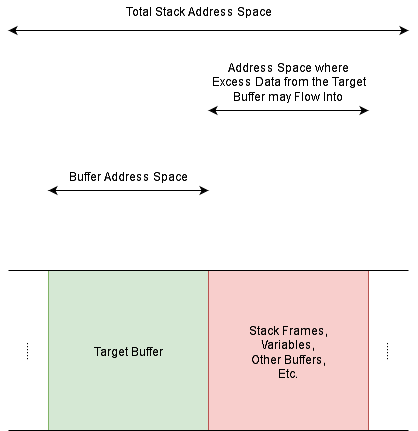
\includegraphics[width=0.4\textwidth]{figures/BufferOverflow.png}}
    \caption{High-level diagram of a buffer overflow.}
    \label{fig:BufferOverflow}
\end{figure}

Figure \ref{fig:BufferOverflow} is a high-level abstraction of a buffer overflow in memory.
It should be noted that the buffer overflow can overwrite parts of a stack frame.
Attackers can intentionally overwrite the return address of the stack frame to redirect a program to malicious code.

One such example of an attack conducted via buffer overflow is an attack on Android's KeyStore service \cite{Hay2014}.
The KeyStore service allows the user to securely store keys for cryptographic operations \cite{AndroidDocs2022Keystore}.
Keys are stored on disk in files containing key as ciphertext (keys are stored in encrypted form).
The keys are identified by filename.
The lack of bounds checking on buffers present in the code (explicitly left out by the KeyStore authors for performance reasons) allows a programmer to inject arbitrary data into the stack memory through the Java API.
By using exploiting this vulnerability, an attacker could inject malicious code that could leak the unencrypted keys.
This attack is particularly damaging to a user, since the keys stored in the KeyStore could be used by applications installed on the device to access sensitive information.

It is difficult to overstate the importance of detecting and patching memory-related vulnerabilities.
Since both the Linux kernel and the native library layers of the Android platform make use of low level languages that tend to allow these vulnerabilities, attacks may be conducted from a multitude of places within the software stack.
Savvy attackers with a robust knowledge of a system's inner workings may find and exploit the vulnerabilities found from reviewing source code.
At the same time, white hat hackers and researchers may also review the code and find vulnerabilities in the code and notify the maintainers so that the code may be patched.
This is the double-edged sword of open source software.

In the meantime, researchers are developing tools to assist in the detection and prevention of memory corruption.
A long-term solution might include the development of more modern, safer programming languages that avoid the classic pitfalls that come with programming applications and libraries in C and C++.
One such example is the Rust programming language, which prevents unsafe memory operations at compile time unless explicitly told to ignore them using the "unsafe" keyword built into the language \cite{Rust2022}.
The "unsafe" keyword has the added benefit of making the code searchable if the aforementioned unsafe operations ultimately do result in exploitable or buggy code.

Other solutions might be the complete isolation of native libraries into a non-privileged environment, as proposed by Sun and Tan \cite{Sun2014}.
Their model proposes the loading of native code into a separate application all on its own that has only the permissions it needs to perform its functions (principle of least privilege).
This limits the scope of the memory the native code has access to, decreasing the threat of memory corruption.
This is an improvement, since normally native code has full access to a device's memory.
It is clear, though, that there is no catch-all solution to fully patch and prevent these exploits in the native libraries (and in the Linux kernel).

\subsection{Application Framework Layer}
The application framework layer consists of a Java API that allows a programmer to access the services provided by the Android platform \cite{AndroidDocs2022Arch}.
Both Linares-Vasquez \etal and Wu \etal report several vulnerabilities in the Activity Manager that exists at this layer \cite{LinaresVasquez2017, Wu2019}.
The activity manager is a service that oversees the application that are actively running on the system.

Armando \etal describe a Denial-of-Service (DoS) attack carried out by Android's Activity Manager \cite{Armando2012}.
The DoS attack effectively creates a fork bomb, filling the device memory space with identical processes until an automatic device reboot is triggered (which would cause an infinite boot loop in the case of the program being run from the bootloader).
The attack exploits the mechanisms through which Android creates new processes via the Activity Manager, which involves interoperating with the Linux kernel layer to create new processes.

Attacks on the Activity manager are a good example of the types of vulnerabilities that may exist in the application framework layer.
Such attacks highlight a particularly unsafe part of the framework, since vulnerabilities here could potentially cause a loss of availability to one or many applications or services.
Other areas of interest might be the telephony API, the built-in web browser, or any other component that facilitates communications and connections (which tend to be vulnerable to man-in-the-middle attacks among others).

\subsection{Application Layer}
The application layer is where the programs accessible by the end user of the device exist.
These applications range from short messaging service (SMS) applications, to web browsers, to calculators.
Applications are allowed to use each other's services in order to reduce the burden on the programmer to provide code for features users would want from an application (such as two-factor authentication, autofill from a password manager, etc.) \cite{AndroidDocs2022Arch}.
Application security in the Android environment is discussed at length in Section IV.
